\documentclass{standalone}
\usepackage{tikz}

\begin{document}

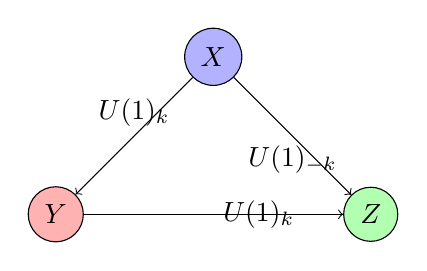
\begin{tikzpicture}[node distance=2cm]

    % Nodes
    \node (A) [circle, draw, fill=blue!30] at (0, 0) {$X$};
    \node (B) [circle, draw, fill=red!30] at (-2, -2) {$Y$};
    \node (C) [circle, draw, fill=green!30] at (2, -2) {$Z$};

    % Arrows
    \draw[->] (A) -- node[above] {$U(1)_k$} (B);
    \draw[->] (A) -- node[below] {$U(1)_{-k}$} (C);
    \draw[->] (B) -- node[right] {$U(1)_k$} (C);

\end{tikzpicture}

\end{document}